\chapter{SGSEAM Evaluation}
\label{cha:ExperimentalDesign}

This chapter describes the experimental design for two assessment tasks: (1) applying the SGSEAM described in \autoref{cha:framework-description} to the Makahiki system described in \autoref{cha:system-description}, (2) applying the SGSEAM to a second IT infrastructure for serious games for sustainability. The goals of these assessments are: (a) obtain insights about
 the strength and weakness of the Makahiki serious game framework we designed and implemented,
 (b) obtain insights about
 the strength and weakness of the second serious game framework,
 (c) obtain insights about the strength and weakness of SGSEAM.

\section{Makahiki Assessment Overview}
The design of assessment of Makahiki using SGSEAM involve: (1) case studies of Makahiki instances in real-world, namely the three Kukui Cup serious games deployed in University of Hawaii at Manoa, Hawaii Pacific University, and East West Center of Hawaii. (2) in-lab experiment of assessing Makahiki system by the students taking the serious game development course in the University of Hawaii at Manoa.

\subsection{Real-world Makahiki Instances Case Studies}

Using the Makahiki as the IT infrastructure, the first and second Kukui Cup Energy challenges at the University of Hawaii were held in 2011 and 2012 for over 1,000 first year students living in the residence halls. Hawaii Pacific University (HPU) held a Kukui Cup Energy challenge in Fall 2012 for about 200 students. An international organization called the East-West Center (EWC) held a Kukui Cup Energy and Water challenge for the international residents living in the residenct halls without smart meters, so the resource consumption data had to be entered by the game mangers manually.

The successful creation of serious game challenges by three different organizations provides evidence that the Makahiki serious game engine can be tailored to the differing needs of separate organizations. First, UH uses smart meters by Electro-Industries Inc., while HPU uses smart meters by EGauge Inc., and EWC collected their energy data manually. Second, while UH and HPU challenges involved only energy consumption data, the EWC challenge involved both energy and water consumption data (which was also collected manually).  Third, the IT infrastructure at UH and HPU provided authentication services using CAS and LDAP, while EWC used the built-in Django authentication. Fourth, the user interface was customized to ``brand'' each challenge with the logo, thematic elements, and the education contents of the sponsoring organizations.

\subsection{In-lab Makahiki Experiment Case Studies}

In Spring 2012, Professor Philip Johnson at the Information and Computer Science Department of University of Hawaii used Makahiki to teach a course in serious game development. The students were seniors or graduate students majoring in computer science related fields. During the course, the students installed Makahiki, designed a serious game instance with Makahiki, and developed an enhancement to the Makahiki system.

These students participated in the assessment experiments of Makahiki, in the aspects of system admin efficiency, game designer efficiency and developer efficiency. The participation is voluntary. This is considered as an in-lab experiment since they are evaluating Makahiki in a class setting and using Makahiki in the development environments.

\section{Makahiki Assessment}
This section describes in details the application of SGSEAM to assess Makahiki using the settings described above.

\subsection{Player assessment}

I plan to apply the SGSEAM player assessment mechanism to the 2011 real-world Kukui Cup instance at the University of Hawaii at Manoa to study the player's experience with the Makahiki framework. There are over 1000 eligible players for this instances. They are the first year college student living in four similar structured resident halls in close vicinity. The challenge lasted for 3 weeks. Makahiki system recorded detailed logging data from every interaction between the players and the website.

To assess the effectiveness of the framework for designing games that improve player literacy in sustainability, we
conducted two energy literacy surveys, one before the challenge (pre-game) and one after
the challenge (post-game). SurveyGizimo is used to create the surveys which consists of the set of sustainability literacy and behavior questionnaires. The response from the two surveys are analyzed to provide insights about the player's literacy and behavior change.

To assess the effectiveness of the framework for designing games that produce positive change in sustainability
behaviors, we recorded and analyzed energy consumption data before, during and after the
challenge.  Before the challenge, an energy usage baseline was established. The energy consumption data is examined to understand any usage pattern or reduction during and after the challenge.

To assess the usability of the game produced by the Makahiki framework, we conducted the in-game usability survey. The survey asked the questions about the players' experience about the user interface of the game. The response from the survey is analyzed to provide insights about the game usability.

In addition to the surveys and energy data measurement, the following engagement metrics will be calculated based on the log data to assess the engagement level of the instance:

\begin{itemize}
\item active participation rate
\item number of players per day
\item average session time
\item submissions per day
\item level of social engagement
\item website errors
\end{itemize}

\subsection{System admin assessment}

There are two approaches described in SGSEAM to assess the game designer's experience: One is the experimental case study that uses the in-lab experiments, another is the interview of the system admin of a real world instance.

In the in-lab experiments, the students in the ICS691 Spring 2013 class were tasked with installing the Makahiki system into their local computers as well as the cloud environment. In order to understand how much time it takes to install the Makahiki and what problems might be encountered, I design a Google form which details the steps of installing Makahiki both locally and in the cloud, and for each step, I ask the students to record the time they spent and the problems they encountered.

Figure \ref{fig:developer-eval-form} illustrates a partial google form used for Makahiki system admin assessment. \autoref{app:googleform} includes the complete google form.
\begin{figure}[ht!]
   \centering
   \includegraphics[height=30em,width=30em]{developer-eval-form.eps}
   \caption{Makahiki Developer assessment Form}
   \label{fig:developer-eval-form}
\end{figure}

The students were also asked to provide feedback about their installation experiences in the form of blog post. In the blog post, I ask them to discuss the following topics:
\begin{itemize}
\item What is the most difficult step during installation?
\item What problems did you encounter during the installation?
\item Have you install any database, web server or similar server products prior to this assignment? Are those installations for development or production purpose?
\item If you have experience installing other servers before, How does your prior experience of installing other servers compare to the installation of Makahiki?
\item What could be improved about the Makahiki installation process?
\item Compare your experience of installing Makahiki in Heroku with installing it locally,
\end{itemize}

The qualitative data collected from the google form response and the blog post from the students will be analyzed to gain insights into how easy it is to install Makahiki, and what contributes to the efficiency of the installation.

In order to gain insights on the experience of a real world system admin who uses the Makahiki, I plan to perform interviews to the system admins of the 2013 Hawaii Pacific University (HPU) challenges.

I will analyze qualitative data collected from the interviews and email changes. The data include:
\begin{itemize}
 \item time taken to install the Makahiki
 \item time taken to maintain the Makahiki, such as backup, monitoring
 \item problems encountered
\end{itemize}

\subsection{Game designer assessment}

There are also two approaches described in SGSEAM to assess the game designer's experience: One is the experimental case study that uses the in-lab experiments, another is the interview of the game designer of a real world instance.

The students in the in-lab experiments were tasked to design a Kukui Cup like serious game using Makahiki. I designed another google form to ask students to follow the designing steps and record their time and problem encountered during their designing process. \autoref{app:googleform} has the complete google form for the steps the students need to follow.

The students were asked to provide feedback about their installation experiences in the form of blog post to discuss the following topics:
\begin{itemize}
\item What is the most difficult step during Challenge Design?
\item What problems did you encounter while designed the challenge?
\item What problems did you encounter while managing the challenge?
\item What could be improved for the Makahiki Challenge Design process?
\item What could be improved for the Makahiki Challenge Management process?
\end{itemize}

I plan to perform interviews to the real world game designers of the 2013 Hawaii Pacific University challenges. We will ask him about his game designing experiences using the Makahiki admin
 interface.

I will analyze both the qualitative data collected from the interviews and email changes with the game designers, and the quantitative collected from the admin interface log data. The qualitative data includes:
\begin{itemize}
    \item How much time did you spend to configure the challenge global settings?
    \item how much time did you spend to setup the player data?
    \item how much time did you spend to design the individual games?
    \item What problem did you encountered?
    \item Did you find it difficult to configure? what is difficult?
    \item Did you find it difficult to design a specific game? which one, what is difficult?
    \item What did you like the least when using the system?
\end{itemize}

The quantitative data includes:
\begin{itemize}
 \item time taken to configure the challenge with regarding to different designing tasks
 \item problems encountered in the log file
\end{itemize}

\subsection{Game manager assessment}
I plan to perform interviews to the real world game managers of the 2013 Hawaii Pacific University challenges to study the experience of the game management using Makahiki.

I will analyze both the qualitative data collected from the interviews and email changes with the game managers, and the quantitative collected from the admin interface log data. The qualitative data includes:
\begin{itemize}
\item How much time did you spend to approving the action submissions?
\item How much time did you spend to monitoring the game status?
\item How much time did you spend to notifying prize winners?
\item What problem did you encountered?
\item Did you find it difficult to manage? what is difficult?
\item What did you like the least when using the system?
\end{itemize}

The quantitative data include:
\begin{itemize}
 \item time taken to manage the challenge with regarding to different managing tasks
 \item problems encountered in the log file
\end{itemize}

\subsection{Developer assessment}

The students in the in-lab experiment are tasked with developing an enhancement to the Makahiki instance. This involves setting up the development environment, following the tutorial to create the "Hello world" widget using Makahiki, and finally, develop the enhancement which extends the functionality of the Makahiki system.

The students are asked to submit their development source code to the public source code repository (Github) and write a blog post to discuss their efforts to complete the development activity.

I will review their source code to compare their code to the reference implementation, analyze the blog post from the students, as well as any email correspondence from students discussing  problems during the development.

\subsection{Preliminary Results}

At the time of the writing of this proposal, I had completed some of the assessments of Makahiki using SGSEAM. The following \autoref{fig:assessment-overview} provides the overview of the status of completed work and the proposed work for applying SGSEAM to Makahiki.

\begin{figure}[ht!]
  \centering
  \begin{tabular}{|c|c|c|c|}
    \hline
    \multicolumn{1}{|p{0.2\columnwidth}|}{\centering\tabhead{Stakeholder}} &
    \multicolumn{1}{|p{0.2\columnwidth}|}{\centering\tabhead{Assessment}} &
    \multicolumn{1}{|p{0.3\columnwidth}|}{\centering\tabhead{Completed}} &
    \multicolumn{1}{|p{0.2\columnwidth}|}{\centering\tabhead{Proposed work}} \\
    \hline
    \multicolumn{1}{|p{0.2\columnwidth}|}{\multirow{2}{*}{Players}} &
    \multicolumn{1}{|p{0.2\columnwidth}|}{Pre Post effectiveness study} &
    \multicolumn{1}{|p{0.3\columnwidth}|}{UH KC 2011 Fall} &
    \multicolumn{1}{|p{0.2\columnwidth}|}{} \\
    \hline
    \multicolumn{1}{|p{0.2\columnwidth}|}{} &
    \multicolumn{1}{|p{0.2\columnwidth}|}{Self-reported usability metrics} &
    \multicolumn{1}{|p{0.3\columnwidth}|}{} &
    \multicolumn{1}{|p{0.2\columnwidth}|}{UH KC 2014} \\
    \cline{2-4}
    \multicolumn{1}{|p{0.2\columnwidth}|}{\multirow{2}{*}{Players}} &
    \multicolumn{1}{|p{0.2\columnwidth}|}{Engagement metrics} &
    \multicolumn{1}{|p{0.3\columnwidth}|}{} &
    \multicolumn{1}{|p{0.2\columnwidth}|}{UH KC 2014} \\
    \hline
    \multicolumn{1}{|p{0.2\columnwidth}|}{\multirow{2}{*}{System admins}} &
    \multicolumn{1}{|p{0.2\columnwidth}|}{In-lab installation study} &
    \multicolumn{1}{|p{0.3\columnwidth}|}{ICS691 2013 Spring} &
    \multicolumn{1}{|p{0.2\columnwidth}|}{} \\
    \cline{2-4}
    \multicolumn{1}{|p{0.2\columnwidth}|}{} &
    \multicolumn{1}{|p{0.2\columnwidth}|}{Post-hoc system admin interview} &
    \multicolumn{1}{|p{0.3\columnwidth}|}{} &
    \multicolumn{1}{|p{0.2\columnwidth}|}{HPU KC 2013 Fall} \\
    \hline
    \multicolumn{1}{|p{0.2\columnwidth}|}{\multirow{2}{*}{Game designers}} &
    \multicolumn{1}{|p{0.2\columnwidth}|}{In-lab game design study} &
    \multicolumn{1}{|p{0.3\columnwidth}|}{ICS691 2013 Spring} &
    \multicolumn{1}{|p{0.2\columnwidth}|}{} \\
    \cline{2-4}
    \multicolumn{1}{|p{0.2\columnwidth}|}{} &
    \multicolumn{1}{|p{0.2\columnwidth}|}{Post-hoc game designer interview} &
    \multicolumn{1}{|p{0.3\columnwidth}|}{} &
    \multicolumn{1}{|p{0.2\columnwidth}|}{HPU KC 2013 Fall} \\
    \hline
    \multicolumn{1}{|p{0.2\columnwidth}|}{\multirow{2}{*}{Game managers}} &
    \multicolumn{1}{|p{0.2\columnwidth}|}{In-lab game management study} &
    \multicolumn{1}{|p{0.3\columnwidth}|}{ICS691 2013 Spring} &
    \multicolumn{1}{|p{0.2\columnwidth}|}{} \\
    \cline{2-4}
    \multicolumn{1}{|p{0.2\columnwidth}|}{} &
    \multicolumn{1}{|p{0.2\columnwidth}|}{Post-hoc game manager interview} &
    \multicolumn{1}{|p{0.3\columnwidth}|}{} &
    \multicolumn{1}{|p{0.2\columnwidth}|}{HPU KC 2013 Fall} \\
    \hline
    \multicolumn{1}{|p{0.2\columnwidth}|}{\multirow{2}{*}{Developers}} &
    \multicolumn{1}{|p{0.2\columnwidth}|}{In-lab game development study} &
    \multicolumn{1}{|p{0.3\columnwidth}|}{ICS691 2013 Spring} &
    \multicolumn{1}{|p{0.2\columnwidth}|}{} \\
    \cline{2-4}
    \multicolumn{1}{|p{0.2\columnwidth}|}{} &
    \multicolumn{1}{|p{0.2\columnwidth}|}{Post-hoc game developer interview} &
    \multicolumn{1}{|p{0.3\columnwidth}|}{} &
    \multicolumn{1}{|p{0.2\columnwidth}|}{UH 2014 Spring} \\
    \hline
  \end{tabular}
  \caption{Status of Makahiki assessment}
  \label{fig:assessment-overview}
\end{figure}


\autoref{app:makahiki-assessment-report} describes the results of the completed assessments of applying SGSEAM to Makahiki.

\section{Lucid Design Dashboard assessment case study}
This section describes the proposed approach to assess the Lucid BuildingOS and BuildingDashboard using the Serious Game Stakeholder Experience Assessment Method (SGSEAM). Lucid BuildingOS and BuildingDashboard provides the software framework to create energy competitions that engage the building occupants to become active participants in energy management \cite{building-dashboard}. The goal of SGSEAM assessment is to identify the major strengths and shortcomings of the framework from the perspectives of user experiences of major stakeholders. The benefits of this assessment are for the developers of the framework to learn from the findings of the assessment and identify any actionable improvements.

\subsection{Step 1: Identify Stakeholders}
Identify the person(s) that use Lucid BuildingOS and BuildingDashboard system and categorize them into SGSEAM stakeholders.

\begin{itemize}
\item Player:
    residents living in the buildings which are participated in the competition

\item System admins:
    IT staffs who are responsible for setting up and maintain the software infrastructure for the competition.
    
\item Game Designers:
    Competition organizers who design/configure the competition to achieve the sustainability goal.
    They may include content experts, instructional designers, etc.

\item Game Managers:
    Competition organizers who is responsible for running the competition
    They may include Residential Life staff, Sustainability Coordinator

\item Game Developers:
    Software developers who use the game framework to customize, extend and enhance their games.    
\end{itemize}

It is desirable to identify the stakeholder persons from different competitions using the same version of the software. For example, many schools will participate in the Campus Conservation National (CCN) 2014. They will use the BuildingOS and BuildingDashboard to create their own competitions. We could select stakeholders from several competitions and use SGSEAM to assess the experiences from them. The more data we collect, the more insights we get.

\subsection{Step 2: Identify Tasks} 
For each stakeholder, identify the tasks that interact with the building OS and building dashboard.

\paragraph{Player:} Interact with the building dashboard interface including:
    \begin{compactitem}
    \item go to the homepage of the competition website
    \item actively look up information about the consumptions of one or several buildings
    \item actively look up standings, prizes
    \item actively participate in the commitments
    \item actively participate in the social sharing
    \end{compactitem}

\paragraph{System admin:} Set up and maintain the software infrastructure:
    \begin{compactitem}
    \item install the software
    \item configuring connectivity with building smart meters if available
    \item backup the data
    \item monitor the performance
    \item scaling the system
    \item patching
    \end{compactitem}
        
\paragraph{Game designer:} Design the competition:
    \begin{compactitem}
    \item Before the competition: use BuildingOS interface to configure and design the competition:\\
        - decide competition period\\
        - set up participant building information (occupancy, energy related LEED certification, manual or automated meters)\\
        - decide baseline period
    
    \item During the competition: monitor competition state, looking up scoreboard info and analytics
    \end{compactitem}

\paragraph{Game manager:} Manage the competition: 
    \begin{compactitem}
    \item enter the data manually in the case of manual meters (at least twice weekly)
    \item manage real world activities, such as events, marketing, handing out prizes
    \item monitor competition state, looking up scoreboard info and analytics
    \end{compactitem}
    
\paragraph{Game Developer:} Use the game framework to customize, extend and enhance their games:
    \begin{compactitem}
    \item use API to get data in and/or out of the system
    \item customize the interface
    \item extend the system to support new meters
    \item enhancement
    \end{compactitem}
    
\subsection{Step 3: Determine assessment approaches}
 Determine the appropriate assessment approaches for each stakeholder and carry out the assessment.

\subsubsection{Player assessment}
 
\paragraph{1. pre-post study:}

One of the goals of the competition is (but not limited to) energy consumption reduction. To assess the effectiveness of this goal, we will need to determine the metrics that may be measured before and 
after the competition to determine the effect of the competition.

Lucid Dashboard calculates percentage of reduction of energy consumption for each participated building, based on the baseline usage of the previous two weeks. 
We could use this metrics at the end of the competition to assess this aspect of the effectiveness of the competition with the respective to the players.
    
\paragraph{2. self-reported metrics: } 

We could conduct a player survey during or after the competition. A number of players (minimum of 20) could be randomly selected to participate in this survey. The survey could be administrated online via tools such as survey monkey. We could design the survey questionnaire as the following:
    
Open-ended questions: 
\begin{compactitem}
\item What did you like most about the website?
\item What did you found confusing?
\item What issues did you have while using the site?
\item What was the thing you liked the least about the site?
\item What can we do to improve the site?\\
\end{compactitem}

Close-ended questions with Likert scale from "Strong disagree" to "Strongly agree": 
\begin{compactitem}
\item It was easy to find what I was looking for on the website
\item The website was responsive 
\item I understood how to play
\item this is something my friends should participate in
\end{compactitem}

Once the survey is created online, the survey administrator could send it out via emails to the selected players with the link to the online survey and the instruction to fill out the survey online.
The survey result will be analyzed to understand the player's experience with the competition interface.
 
\paragraph{3. engagement metrics: }

This approach will gather the website usage data, which requires detailed logging of user interaction within the website. These logging includes http web server logs and/or user action logs which identify every user click on the web page. By using this website usage data, we could calculate the following metrics:

\begin{compactitem}
\item  number of players per day
\item  play time of a player per day
\item  commitment submissions of all player per day
\item  social interaction of all player per day
\item  website errors per day
\end{compactitem}

Distribution of the above metrics across of the period of the competition could provide insights on 
the extent of engagement in different time of the competition. For example, it may be typical that
the first few days of the competition may have higher engagement metrics because of the launch. Another
example of engagement metrics spur could be an announcement of an interesting real-world event. 
    
\subsubsection{System admin assessment}

Due to the cost of recruiting testing subjects and set up the experiments, in-lab experiment assessment may not be appropriate in our case. Instead, we recommend to system admin interview approach. Once we identify the contact info of the system admin of the system, the interview could be administrated by using an online questionnaire form followed by an optional phone interview if needed. We could design the interview with the following questionnaire:

\begin{compactitem}
\item How much time did you spend to install the system and the dependencies?
\item How much time did you spend to configure the meters?
\item How much time did you spend to maintain the system such as backup, patching, monitoring?
\item Did you need to scale the system? if Yes, how much time did you spend?
\item What problems did you encounter?
\item Did you find it difficult to admin the system? What was difficult?
\item Do you agree for us to call you for a short phone interview if we have more questions regarding your experience with the system?
\end{compactitem}

\subsubsection{Game designer assessment}
Similar to system admin assessment, we choose interview approach for game designer assessment. The interview could be administrated by using an online questionnaire form followed by an optional phone interview if needed. Several game designers of different competitions could be contacted for this interview. The more data we collect, the more insights we get. The interview could be designed with the following questionnaire:

\begin{compactitem}
\item How much time did you spend to set up the buildings including meters?
\item How much time did you spend to setup the competition (competition periods, baseline period, participants)?
\item How much time did you spend to setup the homepage by deciding which widgets to include?
\item How much time did you spend to monitor analytical data to understand the state of the game
\item What problems did you encounter?
\item Did you find it difficult to use the interface? What was difficult?
\item Do you agree for us to call you for a short phone interview if we have more questions regarding your experience with the system?
\end{compactitem}
    
\subsubsection{Game manager assessment}

Similar to game designer assessment, we choose interview approach for game manager assessment. The interview could be administrated by using an online questionnaire form followed by an optional phone interview if needed. Several game managers of different competitions could be contacted for this interview. The more data we collect, the more insights we get. The interview could be designed with the following questionnaire: 

\begin{compactitem}
\item How much time did you spend to enter the meter data manually for the baseline period?
\item How much time did you spend to enter the meter data manually for the competition period?    
\item What problems did you encounter?
\item How much time did you spend to monitor analytical data to understand the state of the game
\item Did you find it difficult to manage? What was difficult?\\
\end{compactitem}
    
\subsubsection{Game developer assessment}

BuildingOS and Dashboard may have APIs for developing apps to tie into the framework. We could use the API to develop an extension or customization of the system, for example, create a new widget to be available in the home page, or support the automated energy data collection from a new type of meter.

We could ask developer(s) to implement such enhancement or customization, using the APIs provided by the framework. The developers could be Lucid internal developers or some one outside of Lucid. After the developers completes the task, we will interview the developers to assess his experience for this development task. The interview could be designed with the following questionnaire:

\begin{compactitem}
\item How much time did you spend developing the customization using the game framework?
\item What problem(s) did you encounter?
\item Did you find it difficult to understand, extend and debug the system? What was difficult?\\
\end{compactitem}    